%
%  PyMC User's Guide
%
%  Created by Chris Fonnesbeck on 2006-05-03.
%  Copyright (c) 2006 . All rights reserved.
%
\documentclass[]{book}

% Use utf-8 encoding for foreign characters
%\usepackage[utf8]{inputenc}

% Setup for fullpage use
\usepackage{fullpage}

% Flexible citation syntax
\usepackage{natbib}
% Uncomment some of the following if you use the features
%
% Running Headers and footers
%\usepackage{fancyheadings}

% Multipart figures
%\usepackage{subfigure}

% More symbols
%\usepackage{amsmath}
%\usepackage{amssymb}
%\usepackage{latexsym}

% Surround parts of graphics with box
\usepackage{boxedminipage}

% Package for including code in the document
\usepackage{listings}

% If you want to generate a toc for each chapter (use with book)
\usepackage{minitoc}

% This is now the recommended way for checking for PDFLaTeX:
\usepackage{ifpdf}

% Enable hyeprlinks
\usepackage[pdfpagemode=FullScreen,colorlinks=true,linkcolor=red]{hyperref}

%\newif\ifpdf
%\ifx\pdfoutput\undefined
%\pdffalse % we are not running PDFLaTeX
%\else
%\pdfoutput=1 % we are running PDFLaTeX
%\pdftrue
%\fi

\ifpdf
\usepackage[pdftex]{graphicx}
\else
\usepackage{graphicx}
\fi
\title{PyMC User's Guide \\
Installation and tutorial}
\author{ Christopher Fonnesbeck }

\date{2006-05-03}

\begin{document}

\ifpdf
\DeclareGraphicsExtensions{.pdf, .jpg, .tif}
\else
\DeclareGraphicsExtensions{.eps, .jpg}
\fi

\maketitle

\tableofcontents

\chapter{Introduction}

Bayesian estimation, particularly using Markov chain Monte Carlo (MCMC), is an increasingly relevant approach to statistical estimation. However, few statistical software packages implement MCMC samplers, and they are non-trivial to code by hand. PyMC is a python module that implements the Metropolis-Hastings algorithm as a python class, and is extremely flexible and applicable to a large suite of problems. PyMC includes methods for summarizing output, plotting, goodness-of-fit and convergence diagnostics.

It is straightforward to code a simple MCMC sampler, using either the Gibbs or Metropolis-Hastings algorithm, in Python (or using a variety of other languages, for that matter). However, more complex models can be tricky to implement, each requiring its own unique sampler. A general, reusable sampler is desirable for use in applications, so that a new sampler need not be coded from scratch for every analysis. PyMC is a \href{http://python.org}{Python} module that provides a MCMC toolkit, making Bayesian simulation models relatively easy to implement. PyMC is not an application per se, but rather a set of classes that relieves users of the need for re-implementing MCMC algorithms and associated utilities, such as plotting and statistical summary. This allows the user to concentrate on important aspects of the problem at hand, rather than the mundane details of statistical simulation.

\chapter{Installation}

PyMC is known to run on Mac OS X, Linux and Windows, but in theory should be able to work on just about any platform for which Python is available (and there are many). Rather than a standalone application, PyMC is simply a \emph{module} for the Python programming language. That is, a set of programming classes that are imported into the Python programming environment for subsequent use. The classes are very general, and can therefore be implemented in a variety of Bayesian analytic tasks. I will describe how to install PyMC using both binary installers (for Mac and Windows) and builds from source code.

Pre-built binary and source distributions of PyMC are available from \href{http://trichech.us}{trichech.us}. There are three PyMC distribution formats provided, each containing the same PyMC module, but targeted for different computing platforms. For Macintosh (OS X) users there is an installer package (.mpkg), for Linux users a compressed tar (.tar.gz) source archive, and for Microsoft Windows a binary executable installer (note that this may not always be the latest version, as PyMC is not specifically developed or tested for Windows).

PyMC requires some prerequisite packages to be present on the system before the PyMC package itself is installed. Fortunately, there are currently only a few dependencies, and all are freely available online.
\begin{itemize}

\item Python version 2.4 or later. I recommend using the \href{http://www.activestate.com/Products/ActivePython/}{ActiveState distributions} for Mac OS X and Linux. Windows users should download and install \href{http://code.enthought.com/enthon/}{Enthought Python}, which contains all of the required packages below. Additionally, the Mac OS X binary distribution of PyMC comes bundled with these prerequisites.

\item FORTRAN and C compilers, preferably G77 and GCC (\emph{i.e.} the GNU compilers), respectively. You may use other compilers, but most have not been tested with PyMC.

\item \href{http://numeric.scipy.org/}{Numpy}, latest version. This is a fundamental scientific programming package for python, which replaces a slew of stand-alone packages (including Numeric) that needed to be installed in the past.

\item \href{http://matplotlib.sourceforge.net/}{Matplotlib} version 0.86 or later. This package is used for plotting of MCMC output.
\end{itemize}


\section{Platform-specific instructions}
\subsection{Mac OS X}

If you double-click the installer package, your archive utility will usually expand the installer from its archive. From here, the prerequisite packages can be installed (by double-clicking the installers and following the on-screen instructions), followed by the PyMC package itself.

If you wish to build and install PyMC from source, first ensure that you are using GCC 3.3 (on newer OS X systems GCC 4.0.1 is the default):
\begin{verbatim}
sudo gcc_select 3.3
\end{verbatim}
Then, untar the source archive, then move into the resulting source directory in the command terminal and type:
\begin{verbatim}
python setup.py build
sudo python setup.py install
\end{verbatim}
The \verb=sudo= command is required to install PyMC into the Python site-packages directory, which should have restricted privileges. You will be prompted for a password, and provided you have superuser privileges, the installation will proceed.

\subsection{Linux}

Unfortunately, binary installers are not currently available for Linux systems, but it is straightforward to build the package yourself. Simply untar the package archive, then move to the resulting archive directory and type:
\begin{verbatim}
python setup.py build
sudo python setup.py install
\end{verbatim}

\subsection{Windows}

Simply double-click the executable installation package, and follow the on-screen instructions.
If you wish to build and install PyMC from source, untar the source archive, then move into the resulting source directory in the command terminal and type:
\begin{verbatim}
python setup.py build --compiler=mingw32 install
\end{verbatim}
This assumes you are using the GCC compiler (recommended). Otherwise, change the --compiler argument accordingly.

\section{Testing the Installation}

If there were no errors in the installation process, it was probably successful. Start python and try importing PyMC\footnote{If you are running from the command line, you may have to move to another directory before running python and importing the PyMC module; for example, switch to your home directory: \textbf{cd \textasciitilde}}
\begin{verbatim}
>>> import PyMC
\end{verbatim}
Once the module has been imported, try running the test:
\begin{verbatim}
>>> PyMC.unittest.main()
\end{verbatim}

This test model estimates the switch point between two rate distributions within a time series of coal mining disasters in the UK. If successful, the test should run two chains for 10000 iterations each, then produce some output. Provided that the test runs without incident, you are now ready to start working with PyMC. The remainder of this document deals with building MCMC models in PyMC. I will touch on some essential theory, but will assume a working knowledge of both basic statistical probability and the Python programming language. If you require an introduction to Python, or a refresher, I recommend the online guide \href{http://www.ibiblio.org/obp/thinkCSpy/index.htm}{``How to Think Like a Computer Scientist: Learning with Python"}. Additionally, there are a number of \href{http://rgruet.free.fr/PQR24/PQR2.4.html}{quick reference} pages available online that summarize most of the common Python syntax. For those who require more statistical preparation, a freely-distributable (GNU public license) text \href{https://www.dartmouth.edu/~chance/teaching_aids/books_articles/probability_book/amsbook.mac.pdf}{``Introduction to Probability''} is available for download in PDF format.

\chapter{Markov chain Monte Carlo}

%MCMC methods are algorithms that sample from probability distributions (\emph{i.e.} Monte Carlo simulation) to yield Markov chains.

\section{Monte Carlo Methods in Bayesian Analysis}

Bayesian model specification often results in posterior forms that are difficult to manipulate analytically. However, it is often possible to generate simulated values that share the distributional properties of the specified posterior. Such simulations may be summarized in such a way that describes the posterior density. For example, consider the expected value of some integral quantity:

\[
E[{\bf x}] = \int_{-\infty}^{\infty} {\bf x} f({\bf x}) d{\bf x}, \qquad
{\bf x} = \{x_1,...,x_k\}
\]

\noindent where $k$ is perhaps very large, making the joint distribution of ${\bf x}$ analytically complex. If we can produce random vectors $\{{\bf x_i}\}$, we can use these values to approximate the unknown integral. This process is known as {\emph Monte Carlo integration}. In general, MC integration says that:

\[
I[a,b] = \int_a^b h(x) f(x) dx
\]

\noindent can be estimated by:

\[
\hat{I}[a,b] = \frac{1}{n}\sum_{i=1}^n h(x_i)
\]

\noindent This estimate is useful because:

\begin{itemize}
\item
By the strong law of large numbers:
\[\hat{I}[a,b] \rightarrow I[a,b] \mbox{with probability 1}\]
\item
Simulation error can be measured and controlled:
\[Var(\hat{I}[a,b]) = \frac{1}{n(n-1)}\sum_{i=1}^n (h(x_i)-\hat{I}[a,b])^2\]
\end{itemize}

Why is this relevant to Bayesian analysis? If we replace $f(x)$ with a posterior, $\pi(\theta|x)$ and make $h(x)$ an interesting function of the unknown parameter, the resulting expectation is that of the posterior of $h(\theta)$:

\[
E[h(\theta|x)] = \int \pi(\theta|x) h(\theta) d\theta \approx \frac{1}{n}\sum_{i=1}^n h(\theta)
\]

\subsection{Rejection Sampling}

Though Monte Carlo integration allows us to estimate integrals that are unassailable by analysis, it relies on the ability to draw samples from the posterior distribution. For known parametric forms, this is not a problem; probability integral transforms or bivariate techniques (e.g Box-Muller method) may be used to obtain samples from uniform pseudo-random variates generated from a computer. Often, however, we cannot readily generate random values from non-standard posteriors. In such instances, we can use rejection sampling to generate samples.

\begin{figure}[ht]
        \begin{center}
        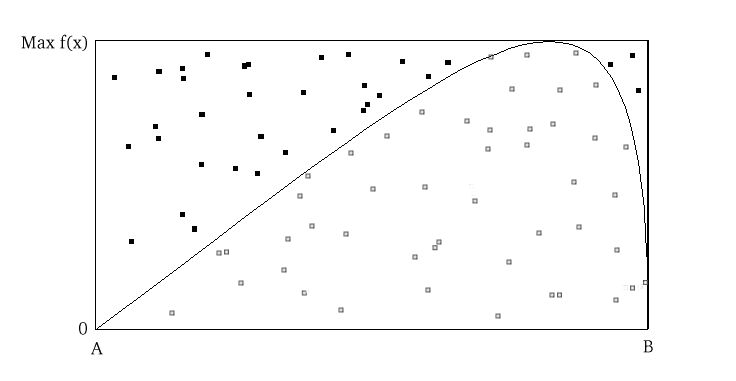
\includegraphics[scale=0.4]{reject.png}
    \end{center}
    \caption{Rejection sampling of a bounded form. Area is estimated by the ratio of accepted (open squares) to total points, multiplied by the rectangle area.}
    \label{fig:bound}
\end{figure}

Posit a function, $f(x)$ which can be evaluated for any value on the support of $x:S_x = [A,B]$, but may not be integrable or easily sampled from. If we can calculate the maximum  value of $f(x)$, we can then define a rectangle that is guaranteed to contain all possible values $(x,f(x))$. It is then trivial to generate points over the box and enumerate the values that fall under the curve (Figure \ref{fig:bound}).

\[
\frac{\mbox{Points under curve}}{\mbox{Points generated}} \times \mbox{box area} = \lim_{n \to \infty} \int_A^B f(x) dx
\]

\begin{figure}[h]
        \begin{center}
        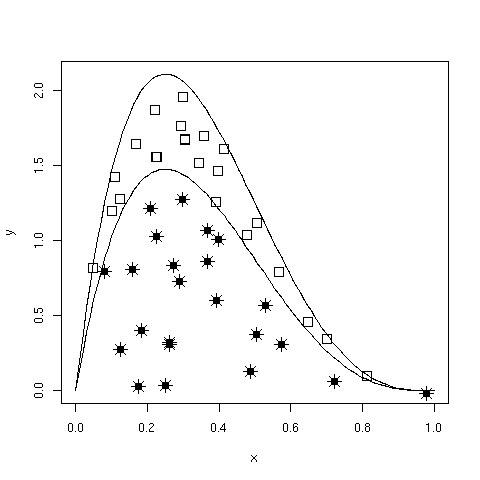
\includegraphics[scale=0.4]{envelope.png}
    \end{center}
    \caption{Rejection sampling of an unbounded form using an enveloping distribution.}
    \label{fig:unbound}
\end{figure}

\noindent This approach is useful, for example, in estimating the normalizing constant for posterior distributions.

If $f(x)$ has unbounded support (i.e. infinite tails), such as a Gaussian distribution, a bounding box is no longer appropriate. We must specify a majorizing (or, enveloping) function, $g(x)$, which implies:

\[
g(x) \le  f(x) \qquad\forall x \in (-\infty,\infty)
\]

Having done this, we can now sample ${x_i}$ from $g(x)$ and accept or reject each of these values based upon $f(x_i)$. Specifically, for each draw $x_i$, we also draw a uniform random variate $u_i$ and accept $x_i$ if $u_i < f(x_i)/kg(x_i)$ (Figure \ref{fig:unbound}). This approach is made more efficient by choosing an enveloping distribution that is ``close'' to the target distribution, thus maximizing the number of accepted points. Further improvement is gained by using optimized algorithms such as importance sampling (see text) which, as the name implies, samples more frequently from important areas of the distribution.

\section{Markov Chains}

A Markov chain is a special type of \emph{stochastic process}. The standard definition of a stochastic process is an ordered collection of random variables:

\[
\{X_t:t \in T\}
\]

\noindent where $t$ is frequently (but not necessarily) a time index. If we think of $X_t$ as a state $X$ at time $t$, and invoke the following dependence condition on each state:

\[
Pr(X_{t+1}=x_{t+1} | X_t=x_t, X_{t-1}=x_{t-1},\ldots,X_0=x_0) = Pr(X_{t+1}=x_{t+1} | X_t=x_t)
\]

\noindent then the stochastic process is known as a Markov chain. This conditioning specifies that the future depends on the current state, but not past states. Thus, the Markov chain wanders about the state space, remembering only where it has just been in the last time step. The collection of transition probabilities is sometimes called a \emph{transition matrix} when dealing with discrete states, or more generally, a \emph{transition kernel}. In the context of Markov chain Monte Carlo, useful to think of the Markovian property as ``mild non-independence''\footnote{In general, for Bayesian analyses, statistical independence is less relevant, relative to classical statistical inference. Instead, we substitute the notion of \emph{exchangeability}, which is a weaker concept, but often just as useful. Exchangeability essentially implies that different permutations (orderings) of a sequence of random variables will have the same marginal distribution. A sequence of random quantities may not be considered independent in a Bayesian sense, but are frequently exchangeable.}. We will see that, while it may be difficult to generate independent samples from a particular posterior distribution, it may be possible to generate dependent samples that may be useful in describing that distribution.

\subsection{Jargon-busting}

Before we move on, it is important to define some general properties of Markov chains. They are frequently encountered in the MCMC literature, and some will help us decide whether MCMC is producing a useful sample from the posterior.

\begin{itemize}
\item \emph{Homogeneity}: A Markov chain is homogeneous at step $t$ if the transition probabilities are independent of the state at $t$. The starting point of the chain is almost never homogeneous, as the initial values are either hand-picked or arbitrary.
\item \emph{Irreducibility}: A Markov chain is irreducible if every state is accessible in one or more steps from any other state. That is, the chain contains no absorbing states. This implies that there is a non-zero probability of eventually reaching state $k$ from any other state in the chain.
\item \emph{Recurrence}: States which are visited repeatedly are \emph{recurrent}. If the expected time to return to a particular state is bounded, this is known as \emph{positive recurrence}, otherwise the recurrent state is \emph{null recurrent}. Further, a chain is \emph{Harris recurrent} when it visits all states $X \in S$ infinitely often in the limit as $t \to \infty$; this is an important characteristic when dealing with unbounded, continuous state spaces. Whenever a chain ends up in a closed, irreducible set of Harris recurrent states, it stays there forever and visits every state with probability one.
\item \emph{Stationarity}: A stationary Markov chain produces the same marginal distribution when multiplied by the transition kernel.  Thus, if $P$ is some $n \times n$ transition matrix:

\[{\bf \pi P} = {\bf \pi}\]

\noindent for Markov chain $\pi$. Thus, $\pi$ is no longer subscripted, and is referred to as the \emph{limiting distribution} of the chain. In MCMC, the chain explores the state space according to its limiting marginal distribution.
\item \emph{Ergodicity}: Ergodicity is an emergent property of Markov chains which are irreducible, positive Harris recurrent and aperiodic. Ergodicity is defined as:

\[
\lim_{n \to \infty} Pr^{(n)}(\theta_i,\theta_j) = \pi(\theta_j) \quad \forall \theta_i, \theta_j \in \Theta
\]

\noindent or in words, the marginal distribution of the chain is the same at one step as at all other steps. This implies that our Markov chain, which we recall is dependent, now generates quantities that are independent. If it means anything to you, ergodicity is the analogue of the strong law of large numbers for Markov chains. For example, take values $\theta_{i+1},\ldots,\theta_{i+n}$ from a chain that has reached an ergodic state. A statistic of interest can then be estimated by:

\[
\hat{h}(\theta) = \frac{1}{n}\sum_{j=i+1}^{i+n} h(\theta_j) \approx h(\theta)
\]

\end{itemize}

\section{Why MCMC Works: Reversible Markov Chains}

Markov chain Monte Carlo simulates a Markov chain for which some function of interest (\emph{e.g.} the joint distribution of the parameters of some model) is the unique, invariant limiting distribution. An invariant distribution with respect to some Markov chain with transition kernel $Pr(y \mid x)$ implies that:
\[
\int_x Pr(y \mid x) \pi(x) dx = \pi(y),
\]
and similarly:
\[
\int_y Pr(x \mid y) \pi(y) dy = \pi(x),
\]

Invariance is guaranteed for any \textbf{reversible} Markov chain. Consider a Markov chain in reverse sequence: $\{\theta^{(n)},\theta^{(n-1)},...,\theta^{(0)}\}$. This sequence is still Markovian, because:
\[
Pr(\theta^{(k)}=y \mid \theta^{(k+1)}=x,\theta^{(k+2)}=x_1,\ldots ) = Pr(\theta^{(k)}=y \mid \theta^{(k+1)}=x)
\]
Forward and reverse transition probabilities may be related through Bayes theorem:
\begin{eqnarray}
Pr(\theta^{(k)}=y \mid \theta^{(k+1)}=x) &=& \frac{Pr(\theta^{(k+1)}=x \mid \theta^{(k)}=y) Pr(\theta^{(k)}=y)}{Pr(\theta^{(k+1)}=x)} \nonumber \\
&=& \frac{Pr(\theta^{(k+1)}=x \mid \theta^{(k)}=y) \pi^{(k)}(y)}{\pi^{(k+1)}(x)} \nonumber
\end{eqnarray}

\[
\frac{Pr(\theta^{(k+1)}=x \mid \theta^{(k)}=y) \pi^{(k)}(y)}{\pi^{(k+1)}(x)}
\]

\noindent Though not homogeneous in general, $\pi$ becomes homogeneous if:
\begin{itemize}
\item $n \rightarrow \infty$
\item $\pi^{(0)}=\pi$ for some $i < k$
\end{itemize}

\noindent If this chain is homogeneous it is called reversible, because it satisfies the \textbf{detailed balance equation}:
\[
\pi(x)Pr(y \mid x) = \pi(y) Pr(x \mid y)
\]
Reversibility is important because it has the effect of balancing movement through the entire state space. When a Markov chain is reversible, $\pi$ is the unique, invariant, stationary distribution of that chain.
Hence, if $\pi$ is of interest, we need only find the reversible Markov chain for which $\pi$ is the limiting distribution. This is what MCMC does!


\section{Gibbs Sampling}

The Gibbs sampler is the simplest and most prevalent MCMC algorithm. It uses samples from conditionally independent distributions to generate a sample from the fully conditional Bayesian posterior. For example, if a posterior has $k$ parameters to be estimated, we may condition each parameter on current values of the other $k-1$ parameters, and sample from the resultant distributional form (usually easier), and repeat this operation on the other parameters in turn. Note that we have now combined Markov chains (conditional independence) and Monte Carlo techniques (estimation by simulation) to yield Markov chain Monte Carlo.

Here is a stereotypical Gibbs sampling algorithm:

\newcounter{lcount}
\begin{list}{\arabic{lcount}}
{\usecounter{lcount}}
\item Choose starting values for states (parameters): ${\bf \theta} = [\theta_1^{(0)},\theta_2^{(0)},\ldots,\theta_k^{(0)}]$
\item Initialize counter $j=1$
\item Draw the following values from each of the $k$ conditional distributions:
\begin{eqnarray*}
\theta_1^{(j)} &\sim& \pi(\theta_1 | \theta_2^{(j-1)},\theta_3^{(j-1)},\ldots,\theta_{k-1}^{(j-1)},\theta_k^{(j-1)}) \\
\theta_2^{(j)} &\sim& \pi(\theta_2 | \theta_1^{(j)},\theta_3^{(j-1)},\ldots,\theta_{k-1}^{(j-1)},\theta_k^{(j-1)}) \\
\theta_3^{(j)} &\sim& \pi(\theta_3 | \theta_1^{(j)},\theta_2^{(j)},\ldots,\theta_{k-1}^{(j-1)},\theta_k^{(j-1)}) \\
\vdots \\
\theta_{k-1}^{(j)} &\sim& \pi(\theta_{k-1} | \theta_1^{(j)},\theta_2^{(j)},\ldots,\theta_{k-2}^{(j)},\theta_k^{(j-1)}) \\
\theta_k^{(j)} &\sim& \pi(\theta_k | \theta_1^{(j)},\theta_2^{(j)},\theta_4^{(j)},\ldots,\theta_{k-2}^{(j)},\theta_{k-1}^{(j)})
\end{eqnarray*}
\item Increment $j$ and repeat until convergence occurs.
\end{list}

As we can see from the algorithm, each distribution is conditioned on the last iteration of its chain values, constituting a Markov chain as advertised. The Gibbs sampler has all of the important properties outlined in the previous section: it is aperiodic, homogeneous and ergodic. Once the sampler converges, all subsequent samples are from the target distribution. This convergence occurs at a geometric rate.

Implementing a simple Gibbs sampler can be done easily in Python. Lets build a Gibbs sampler for estimating a single parameter; for example, simulating from a binomial distribution with a beta prior for $p$ (we assume $n$ is known). We just need a random number generator and a simple loop to iterate over each parameter:
\vspace{1cm}
\begin{verbatim}
# Import random number generators
from numpy import random
beta = random.beta
binomial = random.binomial

# Number of iterations
k=1000

# Prior parameter values
n=20
a=1
b=2

# Some fake data
data = [6,8,4,9,9,7,12]

# Empty arrays to store output
plist = []
ylist = []

# Here's the sampler
for i in range(k):

     # Sample from beta distribution
    p = beta(a+sum(data), len(data)*n-sum(data)+b)

    # Sample from binomial distribution
    y = binomial(n,p)

     # Append samples to lists
    plist.append(p)
    ylist.append(y)

# Calculate medians
plist.sort()
ylist.sort()
pmed = (plist[k/2]+plist[k/2+1])/2
ymed = (ylist[k/2]+ylist[k/2+1])/2

# Print results
print pmed, ymed
\end{verbatim}
\vspace{1cm}

\section{The Metropolis-Hastings Algorithm}

The key to success in applying the Gibbs sampler to the estimation of Bayesian posteriors is being able to specify the form of the complete conditionals of ${\bf \theta}$. In fact, the algorithm cannot be implemented without them. Of course, the posterior conditionals cannot always be neatly specified. The Metropolis-Hastings algorithm, which is implemented by PyMC, rather than generating values from the full set of conditionals, generates candidate state transitions from an alternate distribution, and accepts or rejects each candidate probabilistically according to a specified acceptance ratio.

Let us first consider a simple Metropolis-Hastings algorithm for a single parameter, $\theta$. If necessary, we can transform $\theta$ so that its distribution $\pi(\theta)$ has support over the real line, $\theta:S_{\theta} = (-\infty,\infty)\}$, facilitating the use of convenient random variables such as the normal. This sampling distribution will be used to produce candidate variables, and is therefore referred to as the \emph{proposal distribution}, $q_t(\theta^{\prime} | \theta)$. That is, the generated value, $\theta^{\prime}$, is a \emph{possible} next value for $\theta$ at step $t+1$. We also need to be able to calculate the probability of moving back to the original value from the candidate, or $q_t(\theta | \theta^{\prime})$. These probabilistic ingredients are used to define an \emph{acceptance ratio}:

\[
a(\theta^{\prime},\theta) = \frac{q_t(\theta^{\prime} | \theta) \pi(\theta^{\prime})}{q_t(\theta | \theta^{\prime}) \pi(\theta)}
\]

\noindent The value of $\theta^{(t+1)}$ is then determined by:

\[
\theta^{(t+1)} = \left\{\begin{array}{l@{\quad \mbox{with prob.} \quad}l}\theta^{\prime} & \min(a(\theta^{\prime},\theta),1) \\ \theta^{(t)} & 1 - \min(a(\theta^{\prime},\theta),1) \end{array}\right.
\]

\noindent This transition kernel implies that movement is not guaranteed at every step. It only occurs if the suggested transition is likely based on the acceptance ratio.

A single iteration of the Metropolis-Hastings algorithm proceeds as follows:

\newcounter{lcount2}
\begin{list}{\arabic{lcount2}}
{\usecounter{lcount2}}
\item Sample $\theta^{\prime}$ from $q(\theta^{\prime} | \theta^{(t)})$.
\item Generate a Uniform[0,1] random variate $u$.
\item If $a(\theta^{\prime},\theta) > u$ then $\theta^{(t+1)} = \theta^{\prime}$, otherwise $\theta^{(t+1)} = \theta^{(t)}$.
\end{list}

\noindent The original form of the algorithm specified by Metropolis required that $q_t(\theta^{\prime} | \theta) = q_t(\theta | \theta^{\prime})$, which reduces $a(\theta^{\prime},\theta)$ to $\pi(\theta^{\prime})/\pi(\theta)$, but this is not necessary. In either case, the state moves to high-density points in the distribution with high probability, and to low-density points with low probability. After convergence, the Metropolis-Hastings algorithm describes the full target posterior density, so all points are recurrent.

\subsection{Random-walk Metropolis-Hastings}

A practical implementation of the Metropolis-Hastings algorithm makes use of a random-walk proposal. Recall that a random walk is a Markov chain that evolves according to:

\begin{eqnarray*}
\theta^{(t+1)} &=& \theta^{(t)} + \epsilon_t \\
\epsilon_t &\sim& f(\phi)
\end{eqnarray*}

As applied to the MCMC sampling, the random walk is used as a proposal distribution, whereby dependent proposals are generated according to:

\[
q(\theta^{\prime} | \theta^{(t)}) = f(\theta^{\prime} - \theta^{(t)}) = \theta^{(t)} + \epsilon_t
\]

Generally, the density generating $\epsilon_t$ is symmetric about zero, resulting in a symmetric chain. Chain symmetry implies that $q(\theta^{\prime} | \theta^{(t)}) = q(\theta^{(t)} | \theta^{\prime})$, which reduces the Metropolis-Hastings acceptance ratio to:

\[
a(\theta^{\prime},\theta) = \frac{\pi(\theta^{\prime})}{\pi(\theta)}
\]

The choice of the random walk distribution for $\epsilon_t$ is frequently a normal or Student's $t$ density, but it may be any distribution that generates an irreducible proposal chain.

An important consideration is the specification of the scale parameter for the random walk error distribution. Large values produce random walk steps that are highly exploratory, but tend to produce proposal values in the tails of the target distribution, potentially resulting in very small acceptance rates. Conversely, small values tend to be accepted more frequently, since they tend to produce proposals close to the current parameter value, but may result in chains that mix very slowly. Some simulation studies suggest optimal acceptance rates in the range of 20-50\%. It is often worthwhile to optimize the proposal variance by iteratively adjusting its value, according to observed acceptance rates early in the MCMC simulation.

\section{MCMC Simulation Output}

Stochastic simulation using any MCMC algorithm generates a set of $n$ samples for each parameter in the joint target distribution, where $n$ is the number of MCMC iterations chosen by the user. This sample is used for inference on the parameters of interest, by calculating sample statistics (\emph{e.g.}, mean, mode, variance, quantiles, credible intervals).

\begin{figure}[ht]
        \begin{center}
        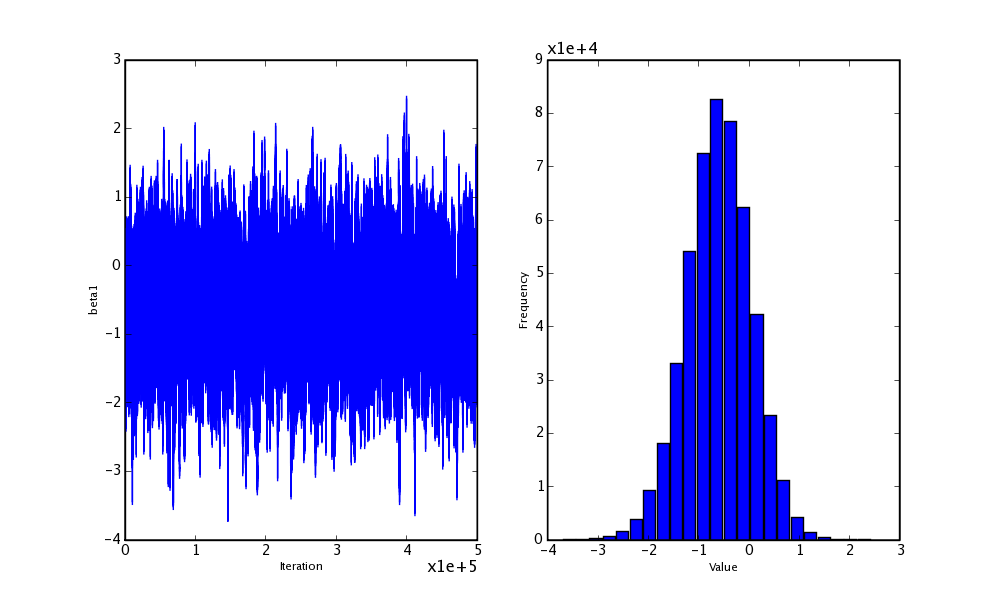
\includegraphics[scale=0.4]{sample_output.png}
    \end{center}
    \caption{Sample trace (left) and histogram (right) from Metropolis-Hastings simulation using PyMC.}
    \label{fig:sample_output}
\end{figure}

Valid inference relies on the assumption that sample values are random (but not necessarily independent) draws from the limiting distribution of the Markov chain. Typically, since unknown parameters are initialized arbitrarily, it is unlikely that the entire sample satisfies this assumption. It is usual, therefore, to discard the first portion of the sample, up to some specified proportion. The appropriate size of this ``burn-in" period is usually determined  \emph{a priori}, sometimes with the assistance of a variety of convergence diagnostics (discussed later). The number of iterations required for convergence varies strongly with the nature of the target posterior distribution and the efficiency of the chosen MCMC algorithm.

Since the sample is derived from a Markov chain, it is necessarily autocorrelated. Poorly-mixing simulations will exhibit autocorrelation more acutely, as successive samples will be relatively close (in parameter space) to their predecessors. Therefore, it is often desirable to ``thin" the sample output, by retaining every $k$ sample from the chain, where $k$ is determined by the severity of the autocorrelation function.

\chapter{Building Models with PyMC}

Programming an effective MCMC algorithm is a non-trivial, time-consuming task for all but the simplest problems. Indeed, building and customizing a sampler by hand for each analysis is inefficient and beyond the programming capabilities of many scientists. However, there are few software packages available that implement such techniques in a way that is accessible to the scientific community. Perhaps the only well-known offering is from the \href{http://www.mrc-bsu.cam.ac.uk/bugs/}{BUGS project}, which maintains and distributes WinBUGS. PyMC offers a very general implementation of a Metropolis-Hastings algorithm that can be used in for estimating a variety of Bayesian models. Since it is simply a Python module (essentially, a tool kit), it can be embedded in a larger analytic framework without moving inputs and results in and out of the programming environment.

PyMC attempts to automate as much of the MCMC analysis as possible. In fact, the end user is responsible for just three tasks when specifying a model:
\begin{itemize}

    \item Data access and manipulation

    \item Parameter and node initialization

    \item Likelihood specification

\end{itemize}

\section{Data Access}\label{sec:data_access}

There are myriad ways of making data available to PyMC. If the amount of the data is small, they may be coded directly in the program itself. For example, here are two lists of values:
\begin{verbatim}
marked = [20,34,13,51,17]

recap = [5,8,3,11,4]
\end{verbatim}
representing marked and recaptured animals, respectively. Alternately, data may be easily read in from a text file. For example, a comma-separated text file like this:
\begin{verbatim}
170102051503,1.3,1.933,0,99.15,L LOST R,MRP,2341,4.1,0.191,2.33,55,1,14,5,3,0,7
170102051503,1.3,1.933,0,99.15,L LOST R,MRP,2350,4.1,0.202,2.52,96.5,1,32,7,12,5,5
170102051503,1.3,1.933,0,99.15,L LOST R,MRP,2374,4.1,0.173,2.5,100,1,23,8,11,9,13
170102051503,1.3,1.933,0,99.15,L LOST R,MRP,2383,4.1,0.185,3.27,79,1,27,4,17,7,19
170102051503,1.3,1.933,0,99.15,L LOST R,MRP,2339,3.8,0.09,2.53,59,1,16,7,17,2,8
170102051503,1.3,1.933,0,99.15,L LOST R,MRP,2340,3.8,0.07,3.55,43.1,1,11,3,10,2,8
170102051503,1.3,1.933,0,99.15,L LOST R,MRP,2343,3.8,0.11,2.5,82,1,49,7,6,3,3
\end{verbatim}
called, for example, mydata.csv, could be imported using the \href{http://docs.python.org/lib/module-csv.html}{csv} module in Python:
\begin{verbatim}
>>> import csv
>>> data = csv.reader(file("mydata.csv"))
>>> for row in data:
...     print row
...
['170102051503', '1.3', '1.933', '0', '99.15', 'L LOST R', 'MRP', '2341', '4.1',
    '0.191', '2.33', '55', '1', '14', '5', '3', '0', '7']
['170102051503', '1.3', '1.933', '0', '99.15', 'L LOST R', 'MRP', '2350', '4.1',
    '0.202', '2.52', '96.5', '1', '32', '7', '12', '5', '5']
['170102051503', '1.3', '1.933', '0', '99.15', 'L LOST R', 'MRP', '2374', '4.1',
    '0.173', '2.5', '100', '1', '23', '8', '11', '9', '13']
['170102051503', '1.3', '1.933', '0', '99.15', 'L LOST R', 'MRP', '2383', '4.1',
    '0.185', '3.27', '79', '1', '27', '4', '17', '7', '19']
['170102051503', '1.3', '1.933', '0', '99.15', 'L LOST R', 'MRP', '2339', '3.8',
    '0.09', '2.53', '59', '1', '16', '7', '17', '2', '8']
['170102051503', '1.3', '1.933', '0', '99.15', 'L LOST R', 'MRP', '2340', '3.8',
    '0.07', '3.55', '43.1', '1', '11', '3', '10', '2', '8']
['170102051503', '1.3', '1.933', '0', '99.15', 'L LOST R', 'MRP', '2343', '3.8',
    '0.11', '2.5', '82', '1', '49', '7', '6', '3', '3']
\end{verbatim}

Data may also be imported directly from a relational database, such as MySQL, PostgreSQL or Oracle. A relational database is the best way to store and manage large quantities of data. Third-party developers offer Python modules to interface with most commercial databases. For example, to query a MySQL database:
\begin{verbatim}
# Connect to database using MySQLdb module for Python
db = MySQLdb.connect(host='fisher.forestry.uga.edu', db='manatee', user='guest', passwd='2phast')
# Create a cursor object to run the query
cur = db.cursor()
# Create query statement
query = 'SELECT * FROM mortality WHERE repyear > 1986'
# Execute query
cur.execute(query)
# Fetch rows
resultset = cur.fetchall()
\end{verbatim}

\section{Parameter Specification}\label{sec:parameter_specification}

Specifying the model parameters and the model likelihood are done by creating a subclass of the main MCMC sampler class in the PyMC module, \verb=MetropolisHastings=. As the name implies, this class is an implementation of a Metropolis-Hastings algorithm, in this case, the random walk algorithm described in the previous section. Subclassing \verb=MetropolisHastings= is simply a matter of specifying two methods (recall that a method is just a function that belongs to a class) within a new class: \verb=__init__= and \verb=calculate_likelihood=. A blank sampler class would look like:

\begin{verbatim}
class MySampler(MetropolisHastings):
    # Note the inheritance of the MetropolisHastings class

    def __init__(self):
          # This  is the initialization function

        # Initialize superclass by calling its __init__ method
        MetropolisHastings.__init__(self)

        # Next, you would specify parameters and nodes

    def calculate_likelihood(self):
        # Specify the joint log-likelihood here

        # Nothing here yet
        pass

\end{verbatim}

The \verb=__init__= method is present in all Python classes, whether specified explicitly or not, and is merely a convention for initializing the class. In the case of \verb=MetropolisHastings=, it is used both to initialize parameters and sometimes to import data. Parameters are specified using the \verb=parameter= method.

\subsubsection*{Method Usage}
\begin{verbatim}
sampler.parameter(name, init_val, discrete=False, dist='normal',
scale=None, random=False, plot=True)
\end{verbatim}

\begin{itemize}

\item \verb=name=: A string containing the name of the parameter.
\item \verb=init_val=: The initial value of the parameter. This may be a scalar- or vector-valued quantity.
\item \verb=discrete= (optional): Flag for specifying parameter as a discrete variable. Valid values include: True, False.
\item \verb=dist= (optional): The proposal distribution for the random walk variate. If not specified, it assumes a normal density.
\item \verb=scale= (optional): A scale parameter associated with the proposal distribution. A larger value confers a larger variance for sampled values. This value will be changed by the algorithm, according to the performance of the sampler.
\item \verb=random= (optional): Specifies parameter as a random effect, and is therefore not counted in AIC calculations. Defaults to False.
\item \verb=plot= (optional): Flags parameter for plotting at the end of the MCMC algorithm. Defaults to True, but one may not always want to plot high-dimension parameters.
\end{itemize}
For example, an array of three recapture probabilities might be initialized by the following method call:
\begin{verbatim}
self.parameter(name='capture', init_val=[0.5,0.5,0.5])
\end{verbatim}

Similarly, nodes, which are variables that are calculated rather than sampled, are declared with a much simpler \verb=node= method, taking only a name as an argument:
\begin{verbatim}
self.node(name='log_capture')
\end{verbatim}

\section{Likelihood Specification}\label{sec:likelihood_specification}

The \verb=calculate_likelihood= method uses the initialized variables and nodes to evaluate a conditional posterior likelihood used to evaluate the current model parameter values. This method employs one or more built-in log-likelihood methods in the \verb=MetropolisHastings= class. The logarithmic form is used in order to allow likelihoods to be added, rather than multiplied; this avoids some numerical problems that pop up from time to time.

These suite of available log-likelihood densities include:
\begin{itemize}

\item \verb=bernoulli_like=: Bernoulli likelihood
\item \verb=beta_like=: Beta likelihood
\item \verb=binomial_like=: Binomial likelihood
\item \verb=cauchy_like=: Cauchy likelihood
\item \verb=chi2_like=: Chi-squared likelihood
\item \verb=dirichlet_like=: Dirichlet likelihood
\item \verb=gamma_like=: Gamma likelihood
\item \verb=geometric_like=: Geometric likelihood
\item \verb=half_normal_like=: Half-normal likelihood
\item \verb=hypergeometric_like=: Hypergeometric likelihood
\item \verb=inverse_gamma_like=: Inverse gamma likelihood
\item \verb=lognormal_like=: Log-normal likelihood
\item \verb=multinomial_like=: Multinomial likelihood
\item \verb=multivariate_hypergeometric_like=: Multivariate hypergeometric likelihood
\item \verb=multivariate_normal_like=: Multivariate normal likelihood
\item \verb=negative_binomial_like=: Negative binomial likelihood
\item \verb=normal_like=: Normal likelihood
\item \verb=poisson_like=: Poisson likelihood
\item \verb=uniform_like=: Uniform likelihood
\item \verb=uniform_mixture_like=: Uniform mixture likelihood
\item \verb=weibull_like=: Weibull likelihood
\item \verb=wishart_like=: Wishart likelihood
\end{itemize}
These methods are available to free the user from having to specify common likelihood functions themselves, and more will be added in the future. They are implemented in FORTRAN, and compiled as Python functions in PyMC using f2py, making them very fast. The formulations of each of these likelihoods is shown in Appendix \ref{chap:statistical_likelihoods}.

By default, \verb=MetropolisHastings= implicitly applies uninformative (i.e. uniform) priors to all parameters. Recall the form of the acceptance ratio:
\[
a(\theta^{\prime},\theta) = \frac{q_t(\theta^{\prime} | \theta) \pi(\theta^{\prime})}{q_t(\theta | \theta^{\prime}) \pi(\theta)}
\]
Note that when $\pi(\theta^{\prime}) = \pi(\theta)$, as is the case for a uniform prior, the acceptance probability reduces to the ratio of the likelihoods.

Users can specify informative priors using any of the available prior methods. For each of the likelihoods outlined above, there is an associated prior. For example, a diffuse gamma prior on some parameter $\theta$ may be specified by:
\begin{verbatim}
self.gamma_prior($\theta$, 0.5, 50)
\end{verbatim}

As an example, lets construct a simple hierarchical regression model in PyMC. Consider a logistic regression, whereby the binomial probability of a particular event $y$ is thought to be a function of some covariate $x$. This model is expressed mathematically as:

\begin{eqnarray*}
    y_t &\sim& \mbox{Bin}(N_t, \pi_t) \\
    \mbox{logit}(\pi_t) &=& \beta_0 + \beta_1 x_t
\end{eqnarray*}
The first step in PyMC is to specify the parameters of the model in the \verb=__init__= method:
\begin{verbatim}

class LogisticSampler(MetropolisHastings):

    def __init__(self):
        # Class initialization

        # Dont forget to initialize the superclass, to get all the
        # MetropolisHastings goodness!
        MetropolisHastings.__init__(self)

        # Intercept
        self.parameter('beta0', init_val=0.0)

        # Slope
        self.parameter('beta1', init_val=0.0)
\end{verbatim}
Next, code the likelihood in \verb=calculate_likelihood=
\begin{verbatim}
    def calculate_likelihood(self):
        # Calculate likelihood, given current parameter values

        # Initialize the likelihood
        like = 0.0

        # Loop over the data
        for x,y,N in data:

            # Calculate probability of event
            pie = self.beta0 + self.beta1 * x

            # Binomial likelihood, given current value of p and data
              like += self.binomial_like(pie, N, y, name="p(y)")

        # Return value (important!)
        return like
\end{verbatim}

Notice that the \verb=binomial_like= method contains a name argument, which identifies that component of the likelihood when goodness-of-fit (GOF) analysis is carried out. This is an optional argument; leaving it blank defaults the name to that of the distribution (\emph{e.g.} \verb=binomial=). Notice that I have assumed that there is an object called \verb=data= that is available to the model, and which contains the input variables. This could be a simple Python \verb=list= object, or a somewhat fancier numpy \verb=array=:

\begin{verbatim}
    data = array([
    [ 11.48,  11.92,  12.29,  14.96, 15.01,
          17.02,  15.90,  20.54, 12.36,  16.55],

        [41, 46, 45, 39, 46, 46, 34, 47, 35, 42],

        [104, 97, 119, 94, 112, 104, 101, 107, 94, 93]
    ])
\end{verbatim}
This is a simple 3 $\times$ 10 array, containing the values for $x$, $y$ and $N$.

Once the data has been made available, the parameters initialized, and the likelihood specified, PyMC takes care of the rest. The model may then be loaded and run:
\begin{verbatim}
>>> import mymodel
>>> sampler = mymodel.LogisticSampler()
>>> sampler.sample(iterations=100000,burn=50000)
\end{verbatim}
This creates an instance of the sampler (here called \verb=sampler=) with a burn-in period of 50000, and runs for 100000 iterations. PyMC will not only give parameter estimates with associated variance and quantile values, but will also plot traces and histograms of each parameter and node. There are a number of optional arguments for \verb=sample=.

\subsubsection{Method Usage}
\begin{verbatim}
sampler.sample(iterations, burn=0, thin=1, tune=True, tune_interval=100,
divergence_threshold=1e10, verbose=True, plot=True, debug=False):
\end{verbatim}
\begin{itemize}

\item \verb=iterations=: Number sampler iterations to run.

\item \verb=burn= (optional): Number of burn-in iterations to discard. Defaults to 0.

\item \verb=thin= (optional): Thinning interval. Defaults to 1 (i.e. no thinning).

\item \verb=tune= (optional): Flag for tuning (i.e. whether to optimize the acceptance probability). Defaults to True.

\item \verb=tune_interval= (optional): Size of interval over which tuning is evaluated. Defaults to 100.

\item \verb=divergence_threshold= (optional): A typically large value that is used to abort models that are obviously diverging.

\item \verb=verbose= (optional): Flag for verbose output. Defaults to True.

\item \verb=plot= (optional): Plotting flag. Defaults to True.

\item \verb=debug= (optional): Flag for debugging using pdb. Defaults to True.
\end{itemize}

\section{Sample Code: Coal mining disasters change point model}

Here is an example using real data. The dataset is a time series of recorded coal mining disasters in the UK from 1851 and 1962. Occurrences of disasters in the time series is thought to be derived from a Poisson process with a large rate parameter in the early part of the time series, and from one with a smaller rate in the later part. We are interested in locating the change point in the series, which perhaps is related to changes in mining safety regulations. This can be implemented as follows:

\begin{verbatim}
    class DisasterSampler(MetropolisHastings):

        def __init__(self):
            """Class initialization"""

            MetropolisHastings.__init__(self)

            # Coal mining disasters per year
            self.data = (4, 5, 4, 0, 1, 4, 3, 4, 0, 6, 3, 3, 4, 0, 2, 6,
                3, 3, 5, 4, 5, 3, 1, 4, 4, 1, 5, 5, 3, 4, 2, 5,
                2, 2, 3, 4, 2, 1, 3, 2, 2, 1, 1, 1, 1, 3, 0, 0,
                1, 0, 1, 1, 0, 0, 3, 1, 0, 3, 2, 2, 0, 1, 1, 1,
                0, 1, 0, 1, 0, 0, 0, 2, 1, 0, 0, 0, 1, 1, 0, 2,
                3, 3, 1, 1, 2, 1, 1, 1, 1, 2, 4, 2, 0, 0, 1, 4,
                0, 0, 0, 1, 0, 0, 0, 0, 0, 1, 0, 0, 1, 0, 1)

            # Switchpoint is specified as a parameter to be estimated
            self.parameter(name='k', init_val=50, discrete=True)

            # Rate parameters of poisson distributions
            self.parameter(name='theta', init_val=array([1.0, 1.0]))

        def calculate_likelihood(self):
            """Likelihood function"""

            # Obtain current values of parameters as local variables
            theta0, theta1 = self.theta
            k = self.k

            # Constrain k
            self.constrain(k, 1, len(self.data)-2)

            # Joint likelihood of parameters based on 2 assumed Poisson densities
            like += self.poisson_like(self.data[:k], theta0, name='early_mean')
            like += self.poisson_like(self.data[k:], theta1, name='late_mean')

            return like
\end{verbatim}
Notice that in this example, unlike the parameters in the logistic regression example earlier, the $theta$ parameters are specified together as an array of length 2. This results in block updating for these parameters, whereby new values for both are proposed and evaluated together. Though either parameterization would be effective in this example, block updating can accelerate convergence for parameters that are thought to be highly correlated. Also notice the use of the $constrain$ method in the likelihood. This prevents parameters from assuming values outside of the specified range. In this case, $k$ is constrained to be within the 2nd (index 1) and penultimate elements in the list; this avoids evaluating either likelihood with no observations.

\section{Model Selection and Random Effects}

PyMC generates two model selection statistics for \verb=MetropolisHastings= models: the Deviance Information Criterion \citep[DIC][]{Spiegelhalter:2002ma} and Akaike’s Information Criterion \citep[AIC][]{Burnham:2002ic}. Both measures use information-theory to give a relative information distance measure from some theoretical, unknown “true” model. Thus, those models with smaller criterion values are thought to be more appropriate models than those with larger values. These criteria balance minimization of model deviance against minimization of the number of parameters included in the model. DIC estimates the “effective” number of parameters, while AIC requires an exact parameter count. For some models (fixed effects), counting parameters is easy, but for models incorporating random effects, it is less clear. One argument simply assumes that individual random effects are not parameters at all, but rather, random draws from populations with their own set of parameters (\emph{i.e.} hyperparameters). To this end, the parameter method allows for a random argument (True or False) that specifies whether the parameter is to be counted as a fixed effect, or not counted, as a random effect.
\begin{verbatim}
self.parameter(name='epsilon', init_val=resize([0.0],100), random=True)
\end{verbatim}

In this example, a 100-element random effect is specified. In turn, this random effect will be modeled as following some distribution (say, normal) with its own location and scale parameters. Thus, AIC will be calculated based on 2 parameters, not 102.

\section{Exporting Output Statistics}

Calling \verb=sample= form any instance of \verb=MetropolisHastings= returns a dictionary (a python look-up table) of summary statistics. This summary dictionary can be used subsequently within a python session, or simply exported using the export method from any \verb=MetropolisHastings= object. This produces a comma-separated values (CSV) text file that may readily be imported into most spreadsheet or database applications.

\subsubsection{Method Usage}
\begin{verbatim}
sampler.export(summary, filename=``pymc", outfile=None)
\end{verbatim}
\begin{itemize}

\item \verb=summary=: A dictionary of summary statistics from the \verb=summary= method.
\item \verb=filename= (optional): Name for output file. Defaults to ‘pymc’.
\item \verb=outfile= (optional): Open file object for output (alternative to filename argument). Defaults to None.
\end{itemize}

\chapter{Diagnostics}

\section{Convergence Diagnostics}

Valid inferences from sequences of MCMC samples are based on the assumption that the samples are derived from the true posterior distribution of interest. Theory guarantees this condition as the number of iterations approaches infinity. It is important, therefore, to determine the minimum number of samples required to ensure a reasonable approximation to the target posterior density. Unfortunately, no universal threshold exists across all problems, so convergence must be assessed independently each time MCMC estimation is performed. The procedures for verifying convergence are collectively known as convergence diagnostics.

One approach to analyzing convergence is analytical, whereby the variance of the sample at different sections of the chain are compared to that of the limiting distribution. These methods use distance metrics to analyze convergence, or place theoretical bounds on the sample variance, and though they are promising, they are generally difficult to use and are not prominent in the MCMC literature. More common is a statistical approach to assessing convergence. With this approach, rather than considering the properties of the theoretical target distribution, only the statistical properties of the observed chain are analyzed. Reliance on the sample alone restricts such convergence criteria to heuristics; that is, convergence cannot be guaranteed. Although evidence for lack of convergence using statistical convergence diagnostics will correctly imply lack of convergence in the chain, the absence of such evidence will not \emph{guarantee} convergence in the chain. Nevertheless, negative results for one or more criteria will provide some measure of assurance to most users that their sample will provide valid inferences.

For most simple models, convergence will occur quickly, sometimes within a the first several hundred iterations, after which all remaining samples of the chain may be used to calculate posterior quantities. For many more complex models, convergence requires a significantly longer burn-in period; sometimes  orders of magnitude more samples are needed. Frequently, lack of convergence will be caused by poor mixing (Figure \ref{fig:mix}). Recall that \emph{mixing} refers to the degree to which the Markov chain explores the support of the posterior distribution. Poor mixing may stem from inappropriate proposals (if one is using the Metropolis-Hastings sampler) or from attempting to estimate models with highly correlated parameters.

\begin{figure}[ht]
\begin{center}
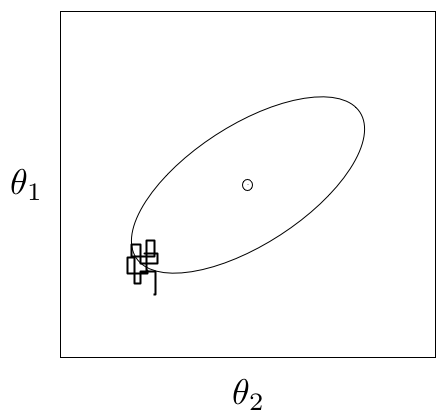
\includegraphics[height=3in]{poor_mixing.png}
\caption{An example of a poorly-mixing sample in two dimensions. Notice that the chain is trapped in a region of low probability relative to the mean (dot) and variance (oval) of the true posterior quantity.}
\label{fig:mix}
\end{center}
\end{figure}

\section*{Informal Methods}

The most straightforward approach for assessing convergence is based on simply plotting and inspecting traces and histograms of the observed MCMC sample. If the trace of values for each of the parameters exhibits asymptotic behaviour\footnote{Asymptotic behaviour implies that the variance and the mean value of the sample stays relatively constant over some arbitrary period.} over the last $m$ iterations, this may be satisfactory evidence for convergence. A similar approach involves plotting a histogram for every set of $k$ iterations (perhaps 50-100) beyond some burn in threshold $n$; if the histograms are not visibly different among the sample intervals, this is reasonable evidence for convergence. Note that such diagnostics should be carried out for each parameter estimated by the MCMC algorithm, because convergent behaviour by one parameter does not imply evidence for convergence for other parameters in the analysis. An extension of this approach can me taken when multiple parallel chains are run, rather than just a single, long chain. In this case, the final values of $c$ chains run for $n$ iterations are plotted in a histogram; just as above, this is repeated every $k$ iterations thereafter, and the histograms of the endpoints are plotted again and compared to the previous histogram. This is repeated until consecutive histograms are indistinguishable.

\begin{figure}[h]
\begin{center}
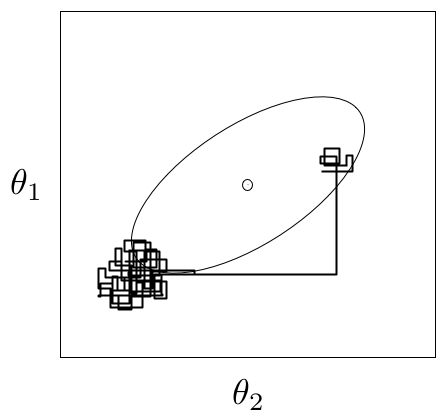
\includegraphics[height=3in]{metastable.png}
\caption{An example of metastability in a two-dimensional parameter space. The chain appears to be stable in one region of the parameter space for an extended period, then unpredictably jumps to another region of the space.}
\label{fig:metas}
\end{center}
\end{figure}

Another \emph{ad hoc} method for detecting convergence is to examine the traces of several MCMC chains initialized with different starting values. Overlaying these traces on the same set of axes should (if convergence has occurred) show each chain tending toward the same equilibrium value, with approximately the same variance. Recall that the tendency for some Markov chains to converge to the true (unknown) value from diverse initial values is called \emph{ergodicity}. This property is guaranteed by the reversible chains constructed using MCMC, and should be observable using this technique. Again, however, this approach is only a heuristic method, and cannot always detect lack of convergence, even though chains may appear ergodic.

A principle reason that evidence from informal techniques cannot guarantee convergence is a phenomenon called metastability. Chains may appear to have converged to the true equilibrium value, displaying excellent qualities by any of the methods described above. However, after some period of stability around this value, the chain may suddenly move to another region of the parameter space (Figure \ref{fig:metas}). This period of metastability can sometimes be very long, and therefore escape detection by these convergence diagnostics. Unfortunately, there is no statistical technique available for detecting metastability.

\section*{Formal Methods}

Along with the \emph{ad hoc} techniques described above, a number of more formal methods exist which are prevalent in the literature. These are considered more formal because they are based on existing statistical methods, such as time series analysis.

PyMC includes one formal convergence diagnostic method, first proposed by \citet{Geweke:1992gm}. This is a time-series approach, which compares the mean and variance of segments from the beginning and end of a single chain.
\begin{equation}
z = \frac{\bar{\theta}_a - \bar{\theta}_b}{\sqrt{Var(\theta_a) + Var(\theta_b)}}
\end{equation}
where $a$ is the early interval and $b$ the late interval. If the z-scores of these two segments are similar, it can provide evidence for convergence. PyMC plots the z-scores of the difference between various initial segments along the chain, and the last 50\% of the remaining chain. If the chain has converged, the majority of points should fall within 2 standard deviations of zero. Calling the convergence method results in a diagnostic plot for each model parameter.

\subsubsection{Method Usage}
\begin{verbatim}
sampler.convergence(first=0.1, last=0.5, intervals=20, burn=0, thin=1, chain=-1, plot=True)
\end{verbatim}
\begin{itemize}

\item \verb=first= (optional): First portion of chain to be used in Geweke diagnostic. Defaults to 0.1 (i.e. first 10% of chain).

\item \verb=last= (optional): Last portion of chain to be used in Geweke diagnostic. Defaults to 0.5 (i.e. last 50% of chain).

\item \verb=intervals= (optional): Number of sub-chains to analyze. Defaults to 20.

\item \verb=burn (optional)=: Number of burn-in iterations to exclude. Defaults to 0 (\emph{i.e.} no burn-in).

\item \verb=thin (optional)=: Thinning factor. Defaults to 1 (\emph{i.e.} no thinning).

\item \verb=chain= (optional): Chain to be analyzed. Defaults to -1 (\emph{i.e}. last chain).

\item \verb=plot= (optional): Plotting flag. Defaults to True.
\end{itemize}
Comprehensive convergence diagnostics are available in the \href{http://lib.stat.cmu.edu/R/CRAN/}{R statistical package}, via the \href{http://www-fis.iarc.fr/coda/}{CODA module}. The \verb=MetropolisHastings= class in PyMC includes a method for exporting model traces in a format that may be directly read by CODA.

\subsubsection{Method Usage}
\begin{verbatim}
sampler.coda_output(filename="coda", burn=0, thin=1)
\end{verbatim}
\begin{itemize}

\item \verb=filename= (optional): Filename of coda output files. Defaults to ``coda''.

\item \verb=burn (optional)=: Number of burn-in iterations to exclude. Defaults to 0 (\emph{i.e.} no burn-in).

\item \verb=thin (optional)=: Thinning factor. Defaults to 1 (\emph{i.e.} no thinning).

\end{itemize}
Calling \verb=coda_output= yields a \verb=.out= file containing raw trace values and a \verb=.ind= file containing indices.

\section{Goodness-of-Fit}

PyMC provides a flexible method for assessing goodness-of-fit (GOF) of models following MCMC estimation. Following \citet{Gelman:1996gp}, the \verb=goodness= method from the \verb=MetropolisHastings= sampler assesses GOF using a simple discrepancy measure for each component of the likelihood. This measure compares the deviance of the data from the expected parameter values to deviance of simulated data from the expected parameter values. Data are simulated based on samples from the trace of all the parameters. These observed and simulated deviances are plotted against one another to yield GOF plots:

Evidence for lack of fit is apparent when points do not fall on either side of the diagonal in approximately the same numbers; the example above shows very good fit. One plot is generated for every component of the likelihood bearing the same name. Additionally, PyMC reports a GOF statistic (which some authors regrettably call the Bayesian $p$-value), which is simply the proportion of points where the simulated deviance is greater than the observed deviance. This value should be close to 0.5 for a well-fit model.

\subsubsection{Method Usage}
\begin{verbatim}
sampler.goodness(iterations, plot=True, loss='squared', burn=0, thin=1, chain=-1, composite=False)
\end{verbatim}

\begin{itemize}

\item \verb=iterations=: Number of GOF iterations to run.

\item \verb=plot (optional)=: Plotting flag. Defaults to True.

\item \verb=loss (optional)=: Loss function to use. Valid arguments include ‘squared’, ‘absolute’ and ‘chi-square’. Defaults to ‘squared’.

\item \verb=burn (optional)=: Number of burn-in iterations to exclude. Defaults to 0 (\emph{i.e.} no burn-in).

\item \verb=thin (optional)=: Thinning factor. Defaults to 1 (\emph{i.e.} no thinning).

\item \verb=chain (optional)=: Chain to be analyzed. Defaults to -1 (\emph{i.e.} last chain).

\item \verb=composite (optional)=: Flag for composite GOF analysis (\emph{i.e.} based on all chains combined). Defaults to False.
\end{itemize}


\subsubsection{Method Usage}
\section{Autocorrelation Plots}

Samples from MCMC algorithms are ususally autocorrelated, due partly to the inherent Markovian dependence structure. The degree of autocorrelation can be quantified using the autocorrelation function:
\begin{eqnarray*}
    \rho_k &=& \frac{\mbox{Cov}(X_t, X_{t+k})}{\sqrt{\mbox{Var}(X_t)\mbox{Var}(X_{t+k})}} \\
            &=& \frac{E[(X_t - \theta)(X_{t+k} - \theta)]}{\sqrt{E[(X_t - \theta)^2] E[(X_{t+k} - \theta)^2]}}
\end{eqnarray*}
The \verb=MetropolisHastings= class includes a method for plotting the autocorrelation function for each parameter in the sampler (Figure \ref{fig:autocorr}). This allows users to examine the relationship among successive samples within sampled chains. Significant autocorrelation suggests that chains require thinning prior to use of the posterior statistics for inference.

\begin{figure}[htbp]
        \begin{center}
        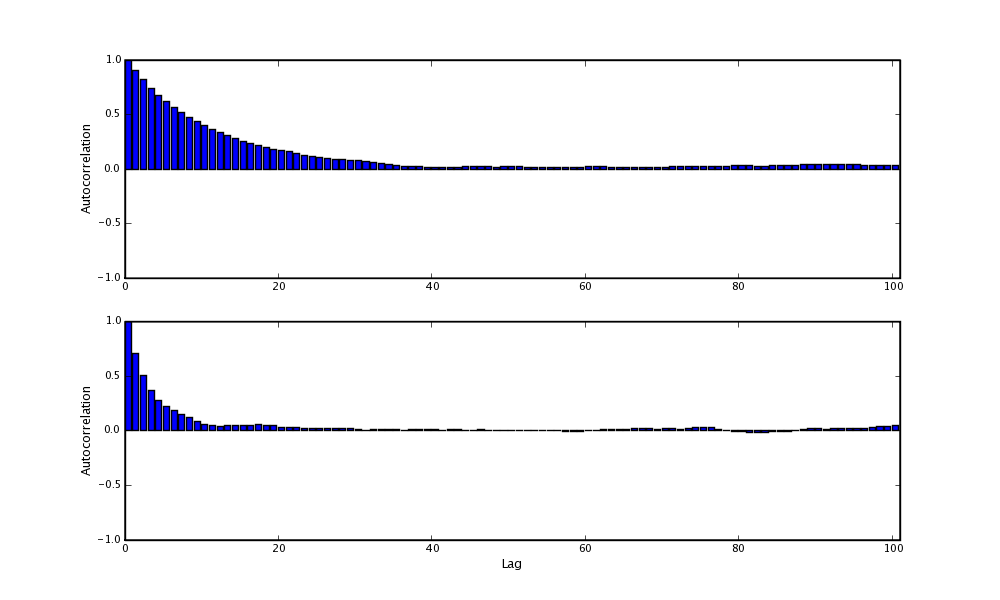
\includegraphics[scale=0.4]{autocorr.png}
    \end{center}
    \caption{Sample autocorrelation plots for two Poisson parameters from coal mining disasters example model.}
    \label{fig:autocorr}
\end{figure}

\begin{verbatim}
sampler.autocorrelation(max_lag=100, burn=0, thin=1, chain=-1)
\end{verbatim}

\begin{itemize}

\item \verb=max_lag (optional)=: Maximum time lag to calculate autocorrelation. Defaults to 100 iterations.

\item \verb=burn (optional)=: Number of burn-in iterations to exclude. Defaults to 0 (\emph{i.e.} no burn-in).

\item \verb=thin (optional)=: Thinning factor. Defaults to 1 (\emph{i.e.} no thinning).

\item \verb=chain (optional)=: Chain to be analyzed. Defaults to -1 (\emph{i.e}. last chain).
\end{itemize}

\bibliographystyle{plainnat}
\bibliography{pymc}

\appendix

\chapter{Statistical Likelihoods}\label{chap:statistical_likelihoods}


\section*{Bernoulli}
\verb=bernoulli_like(x, p)=
\begin{eqnarray*}
f(x \mid p) &=& p^{x- 1} (1-p)^{1-x} \\
\\
&&0 < p < 1 \\
&&x=0,1
\end{eqnarray*}

\section*{Beta}
\verb=beta_like(x, =$\alpha$\verb=, =$\beta$\verb=)=
\begin{eqnarray*}
f(x \mid \alpha, \beta) &=& \frac{\Gamma(\alpha + \beta)}{\Gamma(\alpha) \Gamma(\beta)} x^{\alpha - 1} (1 - x)^{\beta - 1} \\
&&0 < x < 1 \\
&&\alpha > 0, \beta > 0
\end{eqnarray*}

\section*{Binomial}
\verb=binomial_like(x, n, p)=
\begin{eqnarray*}
f(x \mid n, p) &=& \frac{n!}{x!(n-x)!}p^x (1-p)^{1-x} \\
\\
&&0 < p < 1 \\
&&x = 0,\ldots,n
\end{eqnarray*}

\section*{Cauchy}
\verb=cauchy_like(x, =$\alpha$\verb=, =$\beta$\verb=)=
\begin{eqnarray*}
f(x \mid \alpha, \beta) &=& \frac{1}{\pi \beta [1 + (\frac{x-\alpha}{\beta})^2]} \\
\vspace{2cm}\\
&& \beta > 0
\end{eqnarray*}

\section*{Chi-squared}
\verb=chi2_like(x, k)=
\begin{eqnarray*}
f(x \mid k) &=& \frac{x^{\frac{k}{2}-1}e^{-2x}}{\Gamma(\frac{k}{2}) \frac{1}{2}^{k/2}} \\
\vspace{2cm}\\
&& x \ge 0 \\
&& k > 0
\end{eqnarray*}

\section*{Dirichlet}
\verb=dirichlet_like(p, =$\theta$\verb=)=
\begin{eqnarray*}
f(\mathbf{p}) &=& \frac{\Gamma(\sum_{i=1}^k \theta_i)}{\prod \Gamma(\theta_i)} \prod_{i=1}^k p_i^{\theta_i - 1}\\
\vspace{2cm}\\
&& 0 < p_i < 1 \\
&& \theta_i > 0
\end{eqnarray*}

\section*{Gamma}
\verb=gamma_like(x, =$\alpha$\verb=, =$\beta$\verb=)=
\begin{eqnarray*}
f(x \mid \alpha, \beta) &=& \frac{x^{\alpha-1}e^{-x/\beta}}{\Gamma(\alpha) \beta^{\alpha}} \\
\vspace{2cm}\\
&& x \ge 0 \\
&& \alpha > 0 \\
&& \beta > 0
\end{eqnarray*}

\section*{Geometric}
\verb=geometric_like(x, p)=
\begin{eqnarray*}
f(x \mid p) &=& p(1-p)^{x-1} \\
&& 0 < p < 1 \\
&& x = 1,2,3,\ldots
\end{eqnarray*}

\section*{Half-normal}
\verb=half_normal_like(x, =$\tau$\verb=)=
\begin{eqnarray*}
f(x \mid \tau) &=& \sqrt{\frac{2\tau}{\pi}} \exp\left\{ {\frac{-x^2 \tau}{2}}\right\} \\
\vspace{3cm}\\
&& x \ge 0 \\
&& \tau > 0
\end{eqnarray*}

\section*{Hypergeometric}
\verb=hypergeometric_like(x,n,m,N)=
\begin{eqnarray*}
f(x \mid n, m, M) &=& \frac{\left(\begin{array}{c}m \\x\end{array}\right) \left(\begin{array}{c}N-m \\n-x\end{array}\right)}{\left(\begin{array}{c}N \\n\end{array}\right)} \\
\vspace{3cm}\\
&& x = 0,1,\ldots,n\\
&& m = 0,1,\ldots,N
\end{eqnarray*}

\section*{Inverse gamma}
\verb=inverse_gamma_like(x,=$\alpha$\verb=,=$\beta$\verb=)=
\begin{eqnarray*}
f(x \mid \alpha, \beta) &=& \frac{x^{-\alpha - 1} e^{-\frac{1}{x\beta}}}{\Gamma(\alpha)\beta^\alpha} \\
\\
&& x \ge 0 \\
&& \alpha > 0 \\
&& \beta > 0
\end{eqnarray*}

\section*{Log-normal}
\verb=log_normal_like(x, =$\mu$\verb=, =$\tau$\verb=)=
\begin{eqnarray*}
f(x \mid \mu, \tau) &=& \sqrt{\frac{\tau}{2\pi}} \exp\left\{ -\frac{\tau}{2} (x-\mu)^2 \right\}\\
\\
&& \tau > 0
\end{eqnarray*}

\section*{Multinomial}
\verb=multinomial_like(x, n, p)=
\begin{eqnarray*}
f(x \mid n, p) &=& \frac{n!}{\prod_{i=1}^k x_i!} \prod_{i=1}^k p_i^{x_i}\\
\\
&& \sum_{i=1}^k x_i=n \\
&& \sum_{i=1}^k p_i=1
\end{eqnarray*}

\section*{Multivariate normal}
\verb=multivariate_normal_like(x, =$\pi$\verb=, =$\tau$\verb=)=
\begin{eqnarray*}
f(x \mid \pi, T) &=& \frac{T^{n/2}}{(2\pi)^{1/2}} \exp\left\{ -\frac{1}{2} (x-\mu)^{\prime}T(x-\mu) \right\}\\
\\
&& \verb=T positive definite=
\end{eqnarray*}

\section*{Multivariate hypergeometric}
\verb=multivariate_hypergeometric_like(x, n, m, N)=
\begin{eqnarray*}
f(x \mid n, m, N) &=& \frac{{\huge \prod}_{i=1}^k \left(\begin{array}{c}m_i \\x_i\end{array}\right)}{\left(\begin{array}{c}N \\n\end{array}\right)} \\
\vspace{3cm}\\
&& \sum_{i=1}^k x_i = n\\
&& \sum_{i=1}^k m_i = N
\end{eqnarray*}

\section*{Negative binomial}
\verb=negative_binomial_like(x, r, p)=
\begin{eqnarray*}
f(x \mid r, p) &=& \frac{(x+r-1)!}{x! (r-1)!} p^r (1-p)^x \\
\\
&&0 < p < 1 \\
&&x = 0,1,2,\ldots \\
&&r=1,2,3,\ldots
\end{eqnarray*}

\section*{Normal}
\verb=normal_like(x, =$\mu$\verb=, =$\tau$\verb=)=
\begin{eqnarray*}
f(x \mid \mu, \tau) &=& \sqrt{\frac{\tau}{2\pi}} \exp\left\{ -\frac{\tau}{2} (x-\mu)^2 \right\}\\
\\
&& \tau > 0
\end{eqnarray*}

\section*{Poisson}
\verb=poisson_like(x, =$\mu$\verb=)=
\begin{eqnarray*}
f(x \mid \mu) &=& \frac{e^{-\mu}\mu^x}{x!}\\
\\
&& \mu > 0\\
&& x = 0,1,2,\ldots
\end{eqnarray*}

\section*{Uniform}
\verb=uniform_like(x, a, b)=
\begin{eqnarray*}
f(x \mid a, b) &=& \frac{1}{b-a}\\
\\
&& a \le x \le b
\end{eqnarray*}

\section*{Uniform mixture}
\verb=uniform_mixture_like(x, a, m, b)=
\begin{eqnarray*}
f(x \mid a, m, b) &=& \left\{\begin{array}{c}\frac{0.5}{m-a}, \hspace{0.1cm} a \le x < m \\
\\
\frac{0.5}{b-m}, \hspace{0.1cm}m \le x \le b \end{array}\right.
\end{eqnarray*}

\section*{Weibull}
\verb=weibull_like(x, =$\alpha$\verb=, =$\beta$\verb=)=
\begin{eqnarray*}
f(x \mid \alpha, \beta) &=& \frac{\alpha x^{\alpha - 1} \exp(-(\frac{x}{\beta})^{\alpha})}{\beta^\alpha} \\
\\
&& x \ge 0 \\
&& \alpha > 0 \\
&& \beta > 0
\end{eqnarray*}

\section*{Wishart}
\verb=wishart_like(X, n, T)=
\begin{eqnarray*}
f(X \mid n, T) &=& {\mid T \mid}^{n/2}{\mid X \mid}^{(n-k-1)/2} \exp\left\{ -\frac{1}{2} Tr(TX) \right\}\\
\\
&& \verb=X,T symmetric and positive definite= \\
&& k = \verb=length=(X)
\end{eqnarray*}

\section*{Wrapped Cauchy}
\verb=wrapped_cauchy_like(x, =$\mu$\verb=, =$\rho$\verb=)=
\begin{eqnarray*}
f(x \mid \mu, \rho) &=& \frac{1-\rho^2}{2\pi [1 + \rho^2 - 2\rho\cos(x-\mu)]} \\
\\
&& 0 \le \mu < 2\pi \\
&& 0 \le \rho \le 1
\end{eqnarray*}

\end{document}
